\title{tikz Tips}

\documentclass[12pt]{article}

\usepackage[dvipsnames]{xcolor}
\usepackage{tikz}

\begin{document}


\subsection*{Concentric circles with different colors and text}

\phantom{spacing}

% Colors require \usepackage[dvipsnames]{xcolor}.
\begin{center}
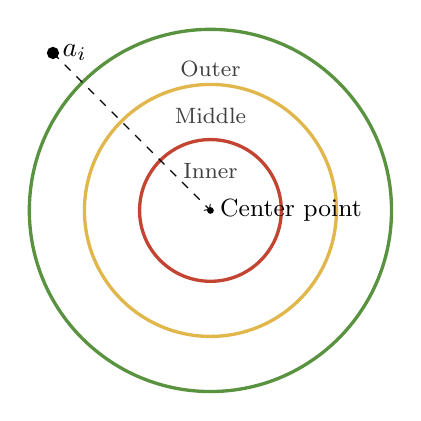
\begin{tikzpicture}

  % 3 circles.
  \filldraw[color=OliveGreen!80, fill=white!5, very thick](0,0) circle (2.3);
  \filldraw[color=Goldenrod!80, fill=white!5, very thick](0,0) circle (1.6);
  \filldraw[color=BrickRed!80, fill=white!5, very thick](0,0) circle (0.9);

  % Text annotations
  \node[align=center, color=darkgray] at (0,1.8) {\footnotesize Outer};
  \node[align=center, color=darkgray] at (0,1.2) {\footnotesize Middle};
  \node[align=center, color=darkgray] at (0,0.5) {\footnotesize Inner};

  % Circle node with text annotation.
  \filldraw[black] (-2,2) circle (2pt) node[anchor=west] {$a_i$};
  
  % Dashed line with arrowhead.
  \draw[dashed,->] (-2,2) -- (0,0);

  % Circle node with text annotation.
  \filldraw[black] (0,0) circle (1pt) node[anchor=west] {\small Center point};

\end{tikzpicture}
\end{center}  


\end{document}
  
